\documentclass[article]{jss}

%%%%%%%%%%%%%%%%%%%%%%%%%%%%%%%%%%%%%%%%%%%%%%%%%%%%%%%%%%%%%%%%%%%%%%%%
% now math stuff and other details...
\usepackage{amsmath,amsthm,amssymb}

%\newtheorem{pro}{Property}[chapter]
%\newtheorem{lem}{Lemma}[chapter]
%\theoremstyle{definition}
%\newtheorem{des}{Definition}[chapter]
%\newtheorem{bsp}{Example}[chapter]
%\newtheorem{remark}{Remark}[chapter]

%\newcommand{\widebar}[1]{\overline{#1}}
\newcommand*\widebar[1]{%
  \vbox{%
    \hrule height 0.5pt%     % Line above with certain width
    \kern0.5ex%             % Distance between line and content
    \hbox{%
      \kern-0.1em%           % Distance between content and left side of box, negative values for lines shorter than content
      \ifmmode#1\else\ensuremath{#1}\fi%  % The content, typeset in dependence of mode
      \kern-0.1em%      % Distance between content and left side of box, negative values for lines shorter than content
    }% end of hbox
  }% end of vbox
}
\def\ds{\displaystyle}
\newcommand{\bed}{\hfill\ensuremath\clubsuit}    % example
\newcommand{\ded}{\hfill\ensuremath\diamondsuit} % definition
\newcommand{\red}{\hfill\ensuremath\heartsuit}   % remark
\newcommand{\rr}[1]{{\ttfamily\slshape\color{DarkGreen} #1}}

\def\baustelle{\includegraphics[height=13.2mm,width=15.6mm]{baustelle.png} }
\def\kleinebaustelle{\includegraphics[height=6.6mm,width=7.8mm]{baustelle.png} }


\newcommand{\fcaption}[2]{\caption{#2 (See \R-Code~{\ref{r#1}}.)}\label{f#1}}
\newcommand{\rcaption}[2]{\caption{#2 (See Figure~{\ref{f#1}}.)}\label{r#1}}
\newcommand{\idea}[1]{\noindent%
\fcolorbox{black}{LightYellow}{\hspace*{1cm}%
\begin{minipage}{\textwidth-2cm-8pt}%{\bf Idea:}\raisebox{1cm}{\,}\vskip5pt\hrule
\vskip15pt#1\raisebox{-4mm}{\,}\end{minipage}%
\hspace*{1cm}}\vskip8mm%
}

\newcommand{\addrscript}[1]{\vspace*{3mm}\R-Code for this chapter: \href{http://www.math.uzh.ch/furrer/download/sta330/chapter#1.R}{www.math.uzh.ch/furrer/download/sta330/chapter#1.R}.}

\makeatletter
%http://tex.stackexchange.com/questions/100139/prevent-equation-labeling-to-change-sizes
  \def\my@tag@font{\small}%normalsize}
  \def\maketag@@@#1{\hbox{\m@th\normalfont\my@tag@font#1}}
  \let\amsmath@eqref\eqref
  \renewcommand\eqref[1]{{\let\my@tag@font\relax\amsmath@eqref{#1}}}
\makeatother


% clever trick to circumvent potential redefines after loading packages:
% \providecommand{\something}{}  % if it does not exist, it creates it.
%      has same syntax as \newcommand
% \renewcommand{\something}{....}
% TUGboat 29(2)


\makeatletter
%umdefinierung exisitierender befehle
\let\oldH\H
\let\oldL\L
\let\oldO\H
\let\oldS\S
\let\olda\a
\let\oldb\b
\let\oldc\c
\let\oldd\d
\let\oldk\k
\let\oldv\v
\let\oldl\l
\let\oldt\t
\let\oldu\u
\let\oldIJ\IJ
\let\oldP\P
\let\P\relax
\let\oldnorm\|

%\DefineVerbatimEnvironment{CodeInput}{Verbatim}{fontshape=sl}
%\DefineVerbatimEnvironment{CodeOutput}{Verbatim}{}

\def\endrem{\hfill$\clubsuit$\\}
\def\endbibrem{\hfill$\spadesuit$\\}


\renewcommand{\|}{|\!|}         % closer norm
\newcommand{\T}{{}^{\top}}%\newcommand{\T}{{}^{\mathsf{T}}}
 
\DeclareMathOperator{\tol}{T}                       % Tolerance reagion
\def\lzwei{\ensuremath{\mathsf{L}_2}} 
\newcommand{\co}{c^{\circ}}
\def\four{^\cF} 
\def\spam{\code{spam}}
\def\R{{\sf R}}
\def\fields{\code{fields}}


%\newtheorem{pro}{Proposition}[chapter]
%\theoremstyle{definition}
%\newtheorem{des}{Definition}[chapter]
%\newtheorem{remark}{Remark}[chapter]
%\newtheorem{bibremark}{Bibliographic Remark}[chapter]
\newcounter{algo}
\newenvironment{algorithm}{%
  \begin{list}{
      (\arabic{algo})
    }{
      \usecounter{algo}
    }%
}{
  \end{list}
}

% some text abbreviation
\newcommand{\GLS}{\text{GLS}}
\newcommand{\GLSE}{\text{GLSE}}
\newcommand{\RR}{\text{RR}}
\newcommand{\OR}{\text{OR}}
\newcommand{\WLS}{\text{WLS}}
\newcommand{\MLE}{\text{MLE}}
\newcommand{\OLS}{\text{OLS}}
\newcommand{\MAE}{\text{MAE}}
\newcommand{\MAD}{\text{MAD}}
\newcommand{\RMSE}{\text{RMSE}}

\newcommand{\ii}{\text{\i}}
\newcommand{\obs}{\text{obs}}

\newcommand{\Bin}{\cB\mathit{\!i\!n}}
\newcommand{\Beta}{\cB\mathit{\!e\!t\!a}}
\newcommand{\Pois}{\cP\mathit{\!o\!i\!s\!s\!o\!n}}
\newcommand{\Exp}{\cE\mathit{\!x\!p}}


%\newcommand\prog[1]{\texttt{#1}}
%\newcommand{\co}{c^{\circ}}
%%%%%%%%%%%%%%%%%% end: maybe to be eliminated

\DeclareMathOperator*{\argmin}{argmin}
\DeclareMathOperator*{\argmax}{argmax}
\DeclareMathOperator{\diag}{diag}
\DeclareMathOperator{\diam}{diam}
\DeclareMathOperator{\card}{card}
\DeclareMathOperator{\cov}{Cov}                   
\DeclareMathOperator{\corr}{Corr}                 
\DeclareMathOperator{\var}{Var}                   
\DeclareMathOperator{\trace}{tr}                  
%\DeclareMathOperator{\E}{E}                       
\DeclareMathOperator{\P}{P}                       
\DeclareMathOperator{\pred}{p}
\DeclareMathOperator{\vect}{vec}                  
\DeclareMathOperator{\vech}{vech}                 
\DeclareMathOperator{\rank}{rank}                 
\DeclareMathOperator{\e}{e}                       
\DeclareMathOperator{\GCV}{GCV}                     
\DeclareMathOperator{\CV}{CV}                     
\DeclareMathOperator{\BLUP}{BLUP}                 
\DeclareMathOperator{\MSE}{MSE}                   
\DeclareMathOperator{\MS}{MS}                   
\DeclareMathOperator{\df}{df}                   
\DeclareMathOperator{\bias}{bias}                   
\DeclareMathOperator{\eig}{eig}                   
\DeclareMathOperator{\Prec}{Prec}
\DeclareMathOperator{\mode}{mode}
\renewcommand{\SS}{\text{SS}}
\renewcommand{\d}{\mathsf{\,d}}

\def\arctanh{\qopname\relax o{arctanh}}  % as in amsopn
\def\atan{\qopname\relax o{atan}}  % as in amsopn
\newcommand{\bigo}{\cO}
\newcommand{\lito}{\text{\scriptsize{$\cO$}}}
\newcommand{\cdfPhi}{\itPhi}
\newcommand{\simiid}{\stackrel[]{\text{iid}}{\sim}}
\newcommand{\ml}{_\text{ML}}

\newcommand*{\stack@relbin}[3][]{%
  \mathop{#3}\limits
  \toks@{#1}%
  \edef\reserved@a{\the\toks@}%
  \ifx\reserved@a\@empty\else_{#1}\fi
  \toks@{#2}%
  \edef\reserved@a{\the\toks@}%
  \ifx\reserved@a\@empty\else^{#2}\fi
  \egroup
}%
\renewcommand*{\stackrel}{\mathrel\bgroup\stack@relbin}
\newcommand*{\stackbin}{\mathbin\bgroup\stack@relbin}


% Kalligraphischer Schriftsatz
\newcommand{\cA}{{\cal{A}}}
\newcommand{\cB}{{\cal{B}}} 
\newcommand{\cC}{{\cal{C}}}
\newcommand{\cD}{{\cal{D}}} 
\newcommand{\cE}{{\cal{E}}}
\newcommand{\cF}{{\cal{F}}}
\newcommand{\cG}{{\cal{G}}}
\newcommand{\cH}{{\cal{H}}}
\newcommand{\cI}{{\cal{I}}}
\newcommand{\cJ}{{\cal{J}}}
\newcommand{\cK}{{\cal{K}}}
\newcommand{\cL}{{\cal{L}}}
\newcommand{\cM}{{\cal{M}}} 
\newcommand{\cN}{{\cal{N}}}
\newcommand{\cO}{{\cal{O}}} 
\newcommand{\cP}{{\cal{P}}}
\newcommand{\cQ}{{\cal{Q}}} 
\newcommand{\cR}{{\cal{R}}} 
\newcommand{\cS}{{\cal{S}}} 
\newcommand{\cT}{{\cal{T}}}
\newcommand{\cU}{{\cal{U}}}
\newcommand{\cV}{{\cal{V}}}
\newcommand{\cW}{{\cal{W}}}
\newcommand{\cX}{{\cal{X}}} 
\newcommand{\cY}{{\cal{Y}}}
\newcommand{\cZ}{{\cal{Z}}} 


\newcommand{\IA}{{\mathbb{A}}}
\newcommand{\IB}{{\mathbb{B}}}
\newcommand{\IC}{{\mathbb{C}}}
\newcommand{\ID}{{\mathbb{D}}}
\newcommand{\IE}{{\mathbb{E}}}
\newcommand{\IF}{{\mathbb{F}}}
\newcommand{\IG}{{\mathbb{G}}}
\newcommand{\IH}{{\mathbb{H}}}
\newcommand{\II}{{\mathbb{I}}}
%\newcommand{\IJ}{{\mathbb{J}}}
\newcommand{\IK}{{\mathbb{K}}}
\newcommand{\IL}{{\mathbb{L}}}
\newcommand{\IM}{{\mathbb{M}}}
\newcommand{\IN}{{\mathbb{N}}}
\newcommand{\IO}{{\mathbb{O}}}
\newcommand{\IP}{{\mathbb{P}}}
\newcommand{\IQ}{{\mathbb{Q}}}
\newcommand{\IR}{{\mathbb{R}}}
\newcommand{\IS}{{\mathbb{S}}}
\newcommand{\IT}{{\mathbb{T}}}
\newcommand{\IU}{{\mathbb{U}}}
\newcommand{\IV}{{\mathbb{V}}}
\newcommand{\IW}{{\mathbb{W}}}
\newcommand{\IX}{{\mathbb{X}}}
\newcommand{\IY}{{\mathbb{Y}}}
\newcommand{\IZ}{{\mathbb{Z}}}


% fette griechische kleinbuchstaben
\newcommand{\balpha}{{\boldsymbol{\alpha}}}
\newcommand{\bbeta}{{\boldsymbol{\beta}}}
\newcommand{\bgamma}{{\boldsymbol{\gamma}}}
\newcommand{\bdelta}{{\boldsymbol{\delta}}}
\newcommand{\blambda}{{\boldsymbol{\lambda}}}
\newcommand{\bepsilon}{{\boldsymbol{\epsilon}}}
\newcommand{\bvarepsilon}{{\boldsymbol{\varepsilon}}}
\newcommand{\bzeta}{{\boldsymbol{\zeta}}}
\newcommand{\bfeta}{{\boldsymbol{\eta}}}  %  <----- exception !
\newcommand{\btheta}{{\boldsymbol{\theta}}{}}
\newcommand{\bvartheta}{{\boldsymbol{\vartheta}}}
\newcommand{\biota}{{\boldsymbol{\iota}}}
\newcommand{\bkappa}{{\boldsymbol{\kappa}}}
\newcommand{\bmu}{{\boldsymbol{\mu}}}
\newcommand{\bnu}{{\boldsymbol{\nu}}}
\newcommand{\bxi}{{\boldsymbol{\xi}}}
\newcommand{\bpi}{{\boldsymbol{\pi}}}
\newcommand{\bvarpi}{{\boldsymbol{\varpi}}}
\newcommand{\brho}{{\boldsymbol{\rho}}}
\newcommand{\bvarrhoi}{{\boldsymbol{\varrho}}}
\newcommand{\bsigma}{{\boldsymbol{\sigma}}}
\newcommand{\bvarsigma}{{\boldsymbol{\varsigma}}}
\newcommand{\btau}{{\boldsymbol{\tau}}}
\newcommand{\bvartau}{{\boldsymbol{\vartau}}}
\newcommand{\bupsilon}{{\boldsymbol{\upsilon}}}
\newcommand{\bphi}{{\boldsymbol{\phi}}}
\newcommand{\bvarphi}{{\boldsymbol{\varphi}}}
\newcommand{\bchi}{{\boldsymbol{\chi}}}
\newcommand{\bpsi}{{\boldsymbol{\psi}}}
\newcommand{\bomega}{{\boldsymbol{\omega}}}


% fette griechische grossbuchstaben
\newcommand{\bGamma}{{\boldsymbol{\Gamma}}}
\newcommand{\bDelta}{{\boldsymbol{\Delta}}}
\newcommand{\bTheta}{{\boldsymbol{\Theta}}}
\newcommand{\bLambda}{{\boldsymbol{\Lambda}}{}}
\newcommand{\bXi}{{\boldsymbol{\Xi}}}
\newcommand{\bPi}{{\boldsymbol{\Pi}}}
\newcommand{\bSigma}{{\boldsymbol{\Sigma}}{}}
\newcommand{\bUpsilon}{{\boldsymbol{\Upsilon}}{}}
\newcommand{\bPhi}{{\boldsymbol{\Phi}}}
\newcommand{\bPsi}{{\boldsymbol{\Psi}}}
\newcommand{\bOmega}{{\boldsymbol{\Omega}}}

% italics griechische grossbuchstaben
\newcommand{\itGamma}{{\mathit{\Gamma}}}
\newcommand{\itDelta}{{\mathit{\Delta}}}
\newcommand{\itTheta}{{\mathit{\Theta}}}
\newcommand{\itLambda}{{\mathit{\Lambda}}}
\newcommand{\itXi}{{\mathit{\Xi}}}
\newcommand{\itPi}{{\mathit{\Pi}}}
\newcommand{\itSigma}{{\mathit{\Sigma}}}
\newcommand{\itUpsilon}{{\mathit{\Upsilon}}}
\newcommand{\itPhi}{{\mathit{\Phi}}}
\newcommand{\itPsi}{{\mathit{\Psi}}}
\newcommand{\itOmega}{{\mathit{\Omega}}}



\newcommand{\A}{{\mathbf{A}}}
\newcommand{\B}{{\mathbf{B}}}
\newcommand{\C}{{\mathbf{C}}}
\newcommand{\D}{{\mathbf{D}}}
\newcommand{\bfE}{{\mathbf{E}}}    % \E: expectation
\newcommand{\F}{{\mathbf{F}}}
\newcommand{\G}{{\mathbf{G}}}
\renewcommand{\H}{{\mathbf{H}}}
\newcommand{\I}{{\mathbf{I}}}
\newcommand{\J}{{\mathbf{J}}}
\newcommand{\K}{{\mathbf{K}}}
\renewcommand{\L}{{\mathbf{L}}}
\newcommand{\bfM}{{\mathbf{M}}}
\newcommand{\N}{{\mathbf{N}}}
\renewcommand{\O}{{\mathbf{O}}}
\newcommand{\bfP}{{\mathbf{P}}}  % \P : probability
\newcommand{\Q}{{\mathbf{Q}}}
\newcommand{\bfR}{{\mathbf{R}}}
\renewcommand{\S}{{\mathbf{S}}}
\newcommand{\bfT}{{\mathbf{T}}} % \T transpose
\newcommand{\U}{{\mathbf{U}}}
\newcommand{\V}{{\mathbf{V}}}
\newcommand{\W}{{\mathbf{W}}}
\newcommand{\X}{{\mathbf{X}}}
\newcommand{\Y}{{\mathbf{Y}}}
\newcommand{\Z}{{\mathbf{Z}}}


\newcommand{\0}{{\mathbf{0}}}
\newcommand{\1}{{\mathbf{1}}}
\newcommand{\2}{{\mathbf{2}}}
\newcommand{\3}{{\mathbf{3}}}
\newcommand{\4}{{\mathbf{4}}}
\newcommand{\5}{{\mathbf{5}}}
\newcommand{\6}{{\mathbf{6}}}
\newcommand{\7}{{\mathbf{7}}}
\newcommand{\8}{{\mathbf{8}}}
\newcommand{\9}{{\mathbf{9}}}

\renewcommand{\a}{{\textbf{\textit{a}}}}
\renewcommand{\b}{{\textbf{\textit{b}}}}
\renewcommand{\c}{{\textbf{\textit{c}}}}
\newcommand{\bfd}{{\textbf{\textit{d}}}}  % \d  'dx'
\newcommand{\bfe}{{\textbf{\textit{e}}}}  % \e  l'exponentiel
\newcommand{\f}{{\textbf{\textit{f}}}}
\newcommand{\g}{{\textbf{\textit{g}}}}
\newcommand{\h}{{\textbf{\textit{h}}}}
\newcommand{\bfi}{{\textbf{\textit{i}}}}%\i  complex i, sans 'dot'
\newcommand{\bfj}{{\textbf{\textit{j}}}}
\renewcommand{\l}{{\textbf{\textit{l}}}}
\renewcommand{\k}{{\textbf{\textit{k}}}}
\newcommand{\m}{{\textbf{\textit{m}}}}
\newcommand{\bfn}{{\textbf{\textit{n}}}}
\newcommand{\bfo}{{\textbf{\textit{o}}}}
\newcommand{\p}{{\textbf{\textit{p}}}}
\newcommand{\q}{{\textbf{\textit{q}}}}
\renewcommand{\r}{{\textbf{\textit{r}}}}
\newcommand{\s}{{\textbf{\textit{s}}}}
\renewcommand{\t}{{\textbf{\textit{t}}}}
\newcommand{\bfu}{{\textbf{\textit{u}}}} %\u used in references
\renewcommand{\v}{{\textbf{\textit{v}}}}
\newcommand{\w}{{\textbf{\textit{w}}}}
\newcommand{\x}{{\textbf{\textit{x}}}}
\newcommand{\y}{{\textbf{\textit{y}}}}
\newcommand{\z}{{\textbf{\textit{z}}}}

% \newcommand{\A}{{\textbf{\textit{A}}}}
% \newcommand{\B}{{\textbf{\textit{B}}}}
% \newcommand{\C}{{\textbf{\textit{C}}}}
% \newcommand{\D}{{\textbf{\textit{D}}}}
% \newcommand{\bfE}{{\textbf{\textit{E}}}}  
% \newcommand{\F}{{\textbf{\textit{F}}}}
% \newcommand{\G}{{\textbf{\textit{G}}}}
% \renewcommand{\H}{{\textbf{\textit{H}}}}
% \newcommand{\I}{{\textbf{\textit{I}}}}
% \newcommand{\J}{{\textbf{\textit{J}}}}
% \newcommand{\K}{{\textbf{\textit{K}}}}
% \renewcommand{\L}{{\textbf{\textit{L}}}}
% \newcommand{\M}{{\textbf{\textit{M}}}}
% \newcommand{\N}{{\textbf{\textit{N}}}}
% \renewcommand{\O}{{\textbf{\textit{O}}}}
% \renewcommand{\P}{{\textbf{\textit{P}}}} 
% \newcommand{\Q}{{\textbf{\textit{Q}}}}
% \newcommand{\R}{{\textbf{\textit{R}}}}
% \renewcommand{\S}{{\textbf{\textit{S}}}}
% \newcommand{\bfT}{{\textbf{\textit{T}}}} % \T transpose
% \newcommand{\U}{{\textbf{\textit{U}}}}
% \newcommand{\V}{{\textbf{\textit{V}}}}
% \newcommand{\W}{{\textbf{\textit{W}}}}
% \newcommand{\X}{{\textbf{\textit{X}}}}
% \newcommand{\Y}{{\textbf{\textit{Y}}}}
% \newcommand{\Z}{{\textbf{\textit{Z}}}}


% \newcommand{\0}{{\textbf{\textit{0}}}}
% \newcommand{\1}{{\textbf{\textit{1}}}}
% \newcommand{\2}{{\textbf{\textit{2}}}}
% \newcommand{\3}{{\textbf{\textit{3}}}}
% \newcommand{\4}{{\textbf{\textit{4}}}}
% \newcommand{\5}{{\textbf{\textit{5}}}}
% \newcommand{\6}{{\textbf{\textit{6}}}}
% \newcommand{\7}{{\textbf{\textit{7}}}}
% \newcommand{\8}{{\textbf{\textit{8}}}}
% \newcommand{\9}{{\textbf{\textit{9}}}}





% \usepackage[utf8]{inputenc}
% \usepackage{listings}
% \usepackage[T1]{fontenc}
% \usepackage{cmbright}
% \usepackage{amsmath}
% \usepackage{amssymb}
% \usepackage{pxfonts}
% \usepackage[sc]{mathpazo}
% \usepackage[T1]{fontenc}
% \usepackage{thumbpdf,lmodern}
% \usepackage{geometry}
% \geometry{verbose,tmargin=2.5cm,bmargin=2.5cm,lmargin=2.5cm,rmargin=2.5cm}
% \setcounter{secnumdepth}{2}
% \setcounter{tocdepth}{2}
% \usepackage{url}
% \usepackage[unicode=true,pdfusetitle,
% bookmarks=true,bookmarksnumbered=true,bookmarksopen=true,bookmarksopenlevel=2,
% breaklinks=false,pdfborder={0 0 1},backref=false,colorlinks=false]
% {hyperref}
% \hypersetup{
% pdfstartview={XYZ null null 1}}
% \usepackage{breakurl}



\DeclareMathOperator{\logit}{logit}
\DeclareMathOperator{\expit}{expit}

\usepackage{natbib}
 
\title{%
  \pkg{causalglm}: A \pkg{tlverse} \proglang{R} package for robust generalized linear models and interpretable causal inference for heterogeneous treatment effects using targeted machine-learning
  }
\Plaintitle{causalglm: robust generalized linear models and interpretable causal inference for heterogeneous treatment effects using targeted machine-learning with the tlverse ecosystem}
\author{Lars van der Laan }
\date{September 2021}

 
  
\Plainauthor{Lars van der Laan }

%% - \title{} in title case
%% - \Plaintitle{} without LaTeX markup (if any)
%% - \Shorttitle{} with LaTeX markup (if any), used as running title
 
\Shorttitle{\pkg{causalglm}: interpretable causal inference for heterogeneous treatment effects}

%% - \Abstract{} almost as usual
\Abstract{
Generalized linear models are well-established and interpretable methods for learning heterogeneous treatment effects. However, conventional parametric generalized linear models make strong parametric assumptions on components of the data-generating distribution that are not directly of interest for the causal question at hand. Notably, in real-world settings, the relation between confounders and the outcome is almost always unknown and may be quite complex. As a result, causal inference based on parametric generalized linear models can be very biased and even misleading. Moreover, in high dimensional settings, generalized linear models and their inference breaks down and alternative methods like lasso and elastic-net regression do not easily provide inference. In this article, we present the \proglang{R} package \pkg{causalglm} that implements robust semiparametric (\textit{spglm}) and nonparametric (\textit{npglm}) generalized linear models and causal inference for heterogeneous treatment effects. These methods utilize targeted maximum likelihood estimation and therefore can leverage adaptive machine-learning algorithms for estimation and variable selection of nonparametric nuisance components of the data-distribution. The methods allow for the interpretable and familiar coefficient-based inference while significantly relaxing the assumptions needed for correct inference through the use of machine-learning. This package supports semiparametric and nonparametric estimation and inference for user-specified parametric models of the estimands: the conditional average treatment effect, the conditional relative risk, the conditional odds ratio, and much more. The nonparametric methods view the user-specified parametric model as a causal approximation (i.e. working-model) and provide interpretable and correct causal inference even when the parametric model is incorrect. Robust causal inference for marginal structural models based on nonparametric projections onto such working models are implemented in the function \textit{msmglm}. A custom lasso-based version of \textit{spglm} is implemented in the function \textit{causalglmnet}, allowing for robust post-confounder-selection causal inference in high dimensions. These methods are implemented using the powerful \pkg{tlverse} machine-learning (\pkg{sl3}) and generalized targeted learning (\pkg{tmle3}) ecosystem.}

%% - \Keywords{} with LaTeX markup, at least one required
%% - \Plainkeywords{} without LaTeX markup (if necessary)
%% - Should be comma-separated and in sentence case.
\Keywords{interpretable-machine-learning, targeted-learning, generalized-linear-models, causal-inference, relative-risk-regression, heterogeneous-treatment-effects, high-dimensional-inference, robust-statistics, semiparametric, nonparametric, double-robust }
\Plainkeywords{interpretable-machine-learning, targeted-learning, generalized-linear-models, causal-inference, relative-risk-regression, heterogeneous-treatment-effects, high-dimensional-inference, robust-statistics, semiparametric, nonparametric, double-robust }


% \usepackage{fancyhdr}          % this and next line are for fancy headers/footers
% \pagestyle{fancy}
\Address{
  Lars van der Laan\\
  Department of Statistics\\
  University of Washington, Seattle\\
  E-mail: \email{vanderlaanlars@yahoo.com}\\
}


\usepackage{Sweave}
\begin{document}
\Sconcordance{concordance:causalglm.tex:causalglm.Rnw:%
1 73 1 1 0 206 1 1 2 1 0 5 1 3 0 1 2 2 1 1 2 1 0 1 8 7 0 1 2 14 0 1 3 1 %
6 5 0 2 1 1 8 7 0 1 2 15 0 1 3 1 1 1 2 20 0 1 2 2 1 1 2 1 0 1 1 1 10 9 %
0 1 1 11 0 1 10 9 0 1 1 11 0 1 10 9 0 1 1 12 0 1 2 3 1 1 7 6 0 1 10 9 0 %
1 1 12 0 1 2 3 1 1 2 1 0 3 1 1 2 1 0 1 1 1 2 1 0 1 10 9 0 1 1 12 0 1 2 %
4 1 1 2 1 0 2 1 1 2 1 0 2 1 5 0 1 8 7 0 1 2 14 0 1 3 1 0 2 1 5 0 1 8 7 %
0 1 2 15 0 1 2 127 1 1 2 1 0 2 1 1 3 1 0 2 1 5 0 1 11 10 0 1 2 11 0 1 2 %
1 0 2 1 5 0 1 8 7 0 1 2 11 0 1 3 1 0 2 1 5 0 1 10 9 0 1 2 15 0 1 1 14 0 %
1 2 1 0 2 1 5 0 1 8 7 0 1 2 14 0 1 3 1 0 2 1 5 0 1 8 7 0 1 2 14 0 1 2 %
19 0 1 2 2 1 1 2 1 0 3 1 1 3 1 0 2 1 1 11 10 0 1 2 16 0 1 1 1 2 1 0 2 1 %
1 9 8 0 1 2 16 0 1 3 1 0 2 1 1 11 10 0 1 2 16 0 1 1 16 0 1 1 1 3 1 0 2 %
1 1 9 8 0 1 2 16 0 1 1 3 0 1 2 4 1 1 2 1 0 4 1 1 3 1 0 2 1 1 8 7 0 1 2 %
1 4 1 0 2 1 1 8 7 0 1 2 1 3 1 0 2 1 1 8 7 0 2 2 4 0 1 3 9 1}

 

\maketitle



\section{Introduction to causalglm}
\subsection{Semiparametric and nonparametric generalized linear models and interpretable causal inference for heterogeneous treatment effects using targeted maximum likelihood estimation}


It is possible to get robust and efficient inference for causal quantities using machine-learning. In the search for answers to causal questions, assuming parametric models can be dangerous. With even a seemingly small amount of confounding and misspecificaton, they can give biased answers. One way of mitigating this challenge is to instead assume a parametric model for only the feature of the data-generating distribution that you care about. That is, assume a semiparametric model! Let the data speak for itself and use machine-learning to model the nuisance features of the data that are not directly related to your causal question. Why worry about things that don't matter for your question? It is not worth the risk of being wrong.

In this package, we utilize targeted machine-learning to generalize the parametric generalized linear models commonly used for heterogeneous treatment effect estimation (e.g. the R package glm) to the world of semi and nonparametric models. There is little-to-no loss in precision/p-values/confidence-interval-widths with these semiparametric methods relative to parametric generalized linear models, but the bias reduction from these methods can be substantial. Simulations suggest that these methods can work well with small sample sizes. All methods utilize targeted maximum likelihood estimation (TMLE) (van der Laan, Rose, 2011).\nocite{vanderLaanRose2011}

Each estimand considered in this package can be modeled with a user-specified parametric model that is either assumed correct (`spglm` and `causalglmnet`) or as an approximation, i.e. working model, of the nonparametric true estimand (`npglm`). The former approach provides interpretable estimates and correct inference only when the parametric model is correct, and the latter approach provides interpretable estimates and nonparametrically correct inference even when the parametric model is incorrect.

By default, the Highly Adaptive Lasso (HAL) and its semiparametric variants are used for estimation. See Benkeser et al. (2016) for an overview of HAL and its statistical performance. For the theoretical analysis of HAL including its fast rate of convergence in high dimensions, see Bibaut et al. (2019) and van der Laan (2017) \nocite{bibaut2019fast}\nocite{HAL2016}\nocite{vanderlaanGenerlaTMLE}. We implement the HAL estimators using the R package hal9001 (Coyle et al., 2021).\nocite{hal1}\nocite{hal2} 
\nocite{vanderlaanGenerlaTMLE} 

Noticable features supported:
\begin{itemize}
\item Efficent semiparametric and nonparametric interpretable inference for user-specified parametric working-models of conditional treatment-effect functions with `spglm` and `npglm`.
\item  Efficient nonparametric inference for marginal structural models for a number of conditional treatment-effect estimands with `npglm`.
\item Designed-easy-to-use interface and built-in machine-learning routines for diverse settings and immediate use.
\item  General machine-learning tools with the tlverse/sl3 generalized machine-learning ecosystem (Coyle et al., 2021).\nocite{coyle2021sl3}
\item  Semiparametric inference with high dimensional covariates and adaptive variable selection of confounders with the wrapper function `causalglmnet`.
\end{itemize}

All functions give the outputs: 
\begin{itemize}
\item Coefficient estimates (and their exponential transform for the OR and RR estimands)
\item 95\% confidence intervals for the coefficients
\item Z-scores and p-values
\item Estimand point-wise predictions and 95\% confidence (prediction) intervals can be extracted with the `predict` function and argument `data`.
\end{itemize}

\subsection{spglm: semiparametric causal inference for generalized linear models}

This function supports semiparametric efficient estimation of following point-treatment estimands:

\begin{itemize}
\item Conditional average treatment effect (CATE). (Causal semiparametric linear regression)
\item Conditional odds ratio (OR) between two binary variables. (Causal semiparametric logistic regression)
\item Conditional relative risk (RR) for nonnegative outcomes and a binary treatment. (Causal semiparametric log-linear relative-risk regression)

\end{itemize}



\subsection{npglm: nonparametric causal inference for generalized linear models}

The function npglm supports nonparametric efficient working-model-based estimation of following point-treatment estimands:

\begin{itemize}
\item Conditional average treatment effect (CATE).
\item Conditional average treatment effect among the treated (CATT)
\item Conditional treatment-specific mean (TSM)
\item Conditional odds ratio (OR) between two binary variables. 
\item Conditional relative risk (RR) for nonnegative outcomes and a binary treatment.  
\end{itemize}

This function also automatically supports marginal structural models by specifying lower dimensional formulas/working-models for the estimands: CATE, CATT, TSM and RR. For ease-of-use, we provide a separate function called "msmglm" for marginal structural model estimation.

\subsection{msmglm: nonparametric causal-inference for marginal structural models}
This function follows user-specified marginal structural models (based on nonparametric projections onto working models) for the following estimands:
\begin{itemize}
\item Marginal structural models for the conditional average treatment effect (CATE).
\item Marginal structural models for the conditional average treatment effect among the treated (CATT).
\item Marginal structural models for the conditional treatment-specific mean (TSM).
\item Marginal structural models for the conditional relative risk (RR). 
\end{itemize}

 

\subsection{causalglmnet: high dimensional causal inference for generalized linear models}
The function causalglmnet supports causal inference with high dimensional confounders for the following estimands:
\begin{itemize}
\item Conditional average treatment effect (CATE). 
\item Conditional odds ratio (OR) between two binary variables. 
\item Conditional relative risk (RR) for nonnegative outcomes and a binary treatment.  
\end{itemize}
Note that the function causalglmnet is a custom wrapper function around the function spglm.

\subsection{npcoxph: assumption-lean inference for the conditional hazard ratio}
The function npcoxph supports the following survival estimands:
\begin{itemize}

\item Nonparametric inference for a user-specified working-model for the conditional hazard ratio between two treatments with `npcoxph`.
\item The estimands supported by `npcoxph` based on lower dimensional formulas can immediately be interpreted as marginal structural models for the hazard ratio.
\end{itemize}





\section{Data-Structure and treatment-effect estimands}

We will mainly consider the point-treatment data-structure $O = (W,A,Y)$ where $W$ represents a vector of baseline covariates (i.e. possible confounders), $A$ is a binary treatment assignment, and $Y$ is some outcome variable. As an example, for a given observation $O$, $W$ could be measurements: age, sex, a risk-score, location, income; $A$ could take the value $1$ if the individual receives the treatment and $0$ if they do not receive the treatment; and $Y$ is a binary or continuous variable that captures the effect of the treatment. For the goal of assessing heterogeneity of the treatment effect, there are a number of popular estimands:

\noindent The conditional average treatment effect (CATE):
\begin{equation}
CATE(w) := E[Y|A=1,W=w] - E[Y|A=0, W=w],
\end{equation}
which is an additive measure of the effect of the treatment ($A=1$) relative to no treatment $(A=0)$.

\vspace{0.5cm}


\noindent The conditional odds ratio (OR) for when $Y$ is binary:
\begin{equation}
OR(w) := \frac{P(Y=1|A=1,W=w)/P(Y=0|A=1,W=w)}{P(Y=1|A=0,W=w)/P(Y=0|A=0,W=w)}
\end{equation}

\vspace{0.5cm}

\noindent The conditional relative risk (RR) for when $Y$ is nonnegative (e.g. a binary or count variable):
\begin{equation}
RR(w) := \frac{E[Y|A=1,W=w]}{E[Y|A=0,W=w]},
\end{equation}
which is a relative measure of the effect of the treatment ($A=1$) relative to no treatment $(A=0)$.

\vspace{0.5cm}

\noindent In some application, non-contrast measures like the conditional treatment-specific mean (TSM) may be of interest:
\begin{equation}
TSM_a(w) := E[Y|A=a,W=w].
\end{equation}

\subsection{Conventional estimators using parametric generalized linear models}
In order to estimate the estimands of the previous section, parametric generalized linear models are often employed (e.g. the R package \textit{glm}). For the CATE,the following linear regression model is often used:
$$E[Y|A, W=w] = \beta_0 A +  \beta_1^T w \cdot A + \beta_2^T w.$$
This model is equivalent to assuming both the nuisance linear model
$$E[Y|A=0,W=w] =  \beta_2^T w$$
and target linear model
$$CATE(w) = \beta_0 + \beta_1^T w.$$
Thus, the coefficient in front of the treatment interactions can be directly interpreted as a measure of the conditional average treatment effect when the parametric model is correct. However, we see that very strong parametric assumptions are made on the orthogonal nuisance function $w \mapsto E[Y|A=0,W=w]$, which has little to do with the CATE.

Next, for the conditional odds ratio, the following logistic regression model is often used
$$\logit \left\{P(Y=1|A,W=w) \right\} =  \beta_0 A +  \beta_1^T w \cdot A + \beta_2^T w.$$
This model is equivalent to assuming both the nuisance logistic model
$$\logit\left\{P(Y=0|A=0,W=w) \right\} =   \beta_2^T w$$
and the target log-linear model
$$\log OR(w) =  \beta_0  +  \beta_1^T w. $$
Once again, we see that the conventional logistic regression model makes strong parametric assumptions on the orthogonal nuisance parameter $P(Y=0|A=0,W=w).$ 

Finally, for the conditional relative-risk, the poisson or log-linear regression model is a well-known approach:
$$\log \left\{E[Y|A,W=w] \right\} =  \beta_0 A +  \beta_1^T w \cdot A + \beta_2^T w.$$
This is equivalent to assuming the nuisance log-linear model
$$\log \left\{E[Y|A=0,W=w] \right\} = \beta_2^T w$$
and the target log-linear model
$$\log \left\{RR(w) \right\} =  \beta_0  +  \beta_1^T w. $$
Besides the strong parametric assumptions on the nuisance parameter $E[Y|A=0,W=w]$, another issue with this approach is that conventional methods only provide inference when the outcome is Poisson distributed, which is not useful if the outcome is binary. Log-link binomial generalized-linear-models are one way to overcome this limitation. 

Under the parametric assumptions, standard generalize linear model software can be used to obtain estimates and inference for the coefficients in the above models for the treatment-effect estimands. However, these methods make much stronger assumptions than are needed. In particular, the parametric assumptions on $E[Y|A=0,W]$ provides little-to-no benefit in interpretability since we are interested in the coefficients for the treatment interaction terms, and it comes at a possibly substantial cost in bias due to model misspecification. Additionally, these methods do not allow for any adaptive estimation of $E[Y|A=0,W]$ (e.g. using the LASSO, variable selection, or machine-learning) and therefore do not perform well in both estimation and inference in high dimensions. In the next section, we consider a partial relaxation of the parametric models through so-called partially-linear generalized linear models.




\section{Semiparametric glms for treatment effect estimation  with spglm}

In this section, we give an overview of semiparametric treatment-effect estimation in partially-linear generalized linear models which allows for adaptive estimation of nuisance parameters of the data-generating distribution that are not directly relevant for the problem at end. Semiparametric models are statistical models in which one component of the data-generating distribution is parametric and the remaining components are nonparametric. For background on semiparametric models and estimators in causal inference, we refer to Bickel et al. (1993) and van der Laan, Robins (2003).\nocite{vanderlaanunified}\nocite{bickel1993efficient}



These methods allow for:
\begin{enumerate}
\item Interpretable (coefficient-based) inference for user-specified parametric models for conditional treatment effect estimands.
\item Adaptive machine-learning and variable selection methods including generalized additive models, LASSO, MARS and gradient-boosting can be used to estimate nuisance parameters nonparametrically, thereby substantially relaxing assumptions for valid inference although still assuming a parametric model for the conditional estimand of interest.
\end{enumerate}

\subsection{Conditional average treatment effect (CATE) and partially-linear least-squares regression}
Let $\underline{f}(w)$ be an arbitrary known vector-valued function of the covariates and consider the linear parametric model $\beta^T \underline{f}(w)$ for $CATE(w)$. The partially-linear least-squares model is of the form:
$$E[Y|A,W=w] = \beta^T \underline{f}(w) \cdot A + h_0(w),$$
where $ h_0(w) := E[Y|A=0,W=w]$ is an unspecified nuisance function that is to be learned from the data nonparametrically. The parametric component of the model is the coefficient vector $\beta$. This model is equivalent to \textit{only} assuming:
$$CATE(w) = \beta^T \underline{f}(w).$$
Thus, this semiparametric model only makes assumptions that directly relate the estimand of interest! 

\noindent A concrete model is choosing $\underline{f}(W) = (1,W)$ which gives the linear model
$$CATE(w) = \beta_0 + \beta_1^T w.$$

Estimates and inference for the coefficient vector in this semiparametric model can be obtained by applying the R function \textit{spglm} with the option `estimand = "CATE"`. We employ machine-learning for initial estimation of the relevant components of the data-generating distribution and then use targeted maximum likelihood estimation for bias-correction, thereby allowing for valid efficient inference. The estimand is estimated using targeted maximum likelihood estimation and the theory and pseudo-code for the method can be found in the working paper, van der Laan (2009). \nocite{OddsRatioreadingsTMLE}

\subsection{Conditional odds ratio (OR) and partially-linear logistic regression}
Let $\underline{f}(w)$ be an arbitrary known vector-valued function of the covariates and consider the parametric model $\beta^T \underline{f}(w)$ for $\log OR(w)$. The partially-linear logistic model is given by:
$$\logit\left\{E[Y|A,W=w]\right\} = \beta^T \underline{f}(w) \cdot A + h_0(w),$$
where $ h_0(w) := \logit\left\{E[Y|A=0,W=w]\right\}$ is an unspecified nuisance function that is to be learned from the data nonparametrically. This model is equivalent to \textit{only} assuming:
$$\log OR(w) = \beta^T \underline{f}(w).$$

Estimates and inference for the coefficient vector in this semiparametric model can be obtained by applying the R function \textit{spglm} with the option `estimand = "OR"`. The estimand is estimated using targeted maximum likelihood estimation and the theory and pseudo-code for the method can be found in the working paper, van der Laan (2009). \nocite{OddsRatioreadingsTMLE}
For a similar estimator based on estimating equations and additional background on the semiparametric logistic regression model, see Tchetgen Tchetgen (2010). \nocite{TchetgenOddsRatio}



\subsection{Conditional relative-risk (RR) and partially-linear log-linear regression}
Let $\underline{f}(w)$ be an arbitrary known vector-valued function of the covariates and consider the parametric model $\beta^T \underline{f}(w)$ for $\log RR(w)$. The partially-linear log-linear model is of the form:
$$\log\left\{E[Y|A,W=w]\right\} = \beta^T \underline{f}(w) \cdot A + h_0(w),$$
where $ h_0(w) := \log\left\{E[Y|A=0,W=w]\right\}$ is an unspecified nuisance function that is to be learned from the data nonparametrically. This model is equivalent to \textit{only} assuming:
$$\log RR(w) =\beta^T \underline{f}(w).$$


Estimates and inference for the coefficient vector in this semiparametric model can be obtained by applying the R function \textit{spglm} with the option `estimand = "RR"`. The estimand is estimated using targeted maximum likelihood estimation and the theory and pseudo-code for the method can be found in the working paper, Tuglus et al. (2011).\nocite{TMLERR} 

\subsection{spglm in action}

Let us generate a mock dataset that has a constant CATE of value 1.
\begin{Schunk}
\begin{Sinput}
> library(causalglm)
> n <- 250
> W <- runif(n, min = -1, max = 1)
> A <- rbinom(n, size = 1, prob = plogis(W))
> Y <- rnorm(n, mean = A + W, sd = 0.3)
> data <- data.frame(W, A, Y)
\end{Sinput}
\end{Schunk}

We specify the parametric form of the CATE through the formula argument. In this case, we will use the intercept-only formula which is equivalent to assuming the CATE is constant.  The output consists of:
a coefficient estimate for the intercept, lower and upper confidence intervals, an asymptotic standard error estimate for the estimator, a Z-score and p-value. The argument `W` should be a character vector of variable names in data for which to adjust, `A` should be the name of a treatment variable, and `Y` should be the name of an outcome variable. We set the argument `estimand = "CATE"` to estimate the conditional average treatment effect.
\begin{Schunk}
\begin{Sinput}
> formula <- ~1
> output <-
+   spglm(
+     formula,
+     data,
+     W = "W", A = "A", Y = "Y",
+     estimand = "CATE",
+     verbose = FALSE
+   )
> summary(output)
\end{Sinput}
\begin{Soutput}
A causalglm fit object obtained from spglm for the estimand CATE with formula: 
CATE(W) = 0.954 * (Intercept)

Coefficient estimates and inference:
   type       param  tmle_est         se     lower    upper  Z_score p_value
1: CATE (Intercept) 0.9542019 0.03807921 0.8795681 1.028836 396.2072       0
\end{Soutput}
\begin{Sinput}
> 
\end{Sinput}
\end{Schunk}
We can also do a much more complex model with higher dimensional treatment effect interactions. The following data distribution has $CATE(w) = 1 + w$.  
\begin{Schunk}
\begin{Sinput}
> Y <-
+   rnorm(n,
+     mean = A * W + A + poly(W, degree = 3) + sin(4 * W),
+     sd = 0.4
+   )
> data <- data.frame(W, A, Y)
> formula <- ~ 1 + W
> output <-
+   spglm(
+     formula,
+     data,
+     W = "W", A = "A", Y = "Y",
+     estimand = "CATE",
+     verbose = FALSE
+   )
> summary(output)
\end{Sinput}
\begin{Soutput}
A causalglm fit object obtained from spglm for the estimand CATE with formula: 
CATE(W) = 1.03 * (Intercept) + 1.06 * W

Coefficient estimates and inference:
   type       param tmle_est         se     lower    upper  Z_score p_value
1: CATE (Intercept) 1.026334 0.05281779 0.9228126 1.129855 307.2404       0
2: CATE           W 1.055546 0.10111576 0.8573626 1.253729 165.0548       0
\end{Soutput}
\begin{Sinput}
> 
\end{Sinput}
\end{Schunk}

We can also obtain predictions and confidence intervals thereof at observations.
\begin{Schunk}
\begin{Sinput}
> head(predict(output, data = data))
\end{Sinput}
\begin{Soutput}
  (Intercept)           W   CATE(W)        se   CI_left  CI_right   Z-score
1           1 -0.37682262 0.6285800 1.0733566 0.4955254 0.7616347  9.259479
2           1  0.82412726 1.8962378 1.4942962 1.7110029 2.0814726 20.064396
3           1 -0.07848771 0.9434862 0.8557327 0.8374085 1.0495639 17.432812
4           1 -0.69953343 0.2879440 1.4555070 0.1075174 0.4683705  3.127978
5           1 -0.20349268 0.8115377 0.9234727 0.6970629 0.9260126 13.894876
6           1 -0.27131286 0.7399504 0.9755089 0.6190251 0.8608758 11.993374
    p-value
1 0.0000000
2 0.0000000
3 0.0000000
4 0.0017601
5 0.0000000
6 0.0000000
\end{Soutput}
\end{Schunk}

Currently, the nonparametric learning is performed using the partially-linear first-order Highly Adaptive Lasso (HAL) implemented using the R package tlverse/hal9001. HAL is an adaptive piece-wise linear regression spline estimator and the custom implementation performs the risk minimization entirely within the semiparametric model. It is implemented using LASSO regression with the parametric treatment interactions (as specified by the formula argument) unpenalized and a rich penalized spline basis for the nonparametric component of the model. This method performs risk minimization entirely within the semiparametric model. There are a number of other built-in learning options: c("HAL", "SuperLearner", "glm", "glmnet", "gam", "mars", "ranger", "xgboost")

\begin{Schunk}
\begin{Sinput}
> Y <- rnorm(n, mean = A * W + A + W, sd = 0.4)
> data <- data.frame(W, A, Y)
> # generalized additive models:
> output <-
+   spglm(
+     formula,
+     data,
+     W = "W", A = "A", Y = "Y",
+     estimand = "CATE",
+     learning_method = "gam",
+     verbose = FALSE
+   )
> summary(output)
\end{Sinput}
\begin{Soutput}
A causalglm fit object obtained from spglm for the estimand CATE with formula: 
CATE(W) = 1 * (Intercept) + 0.866 * W

Coefficient estimates and inference:
   type       param  tmle_est         se     lower    upper  Z_score p_value
1: CATE (Intercept) 1.0031337 0.04799965 0.9090561 1.097211 330.4386       0
2: CATE           W 0.8664897 0.08372657 0.7023887 1.030591 163.6327       0
\end{Soutput}
\begin{Sinput}
> # multivariate adaptive regression splines:
> output <-
+   spglm(
+     formula,
+     data,
+     W = "W", A = "A", Y = "Y",
+     estimand = "CATE",
+     learning_method = "mars",
+     verbose = FALSE
+   )
> summary(output)
\end{Sinput}
\begin{Soutput}
A causalglm fit object obtained from spglm for the estimand CATE with formula: 
CATE(W) = 1 * (Intercept) + 0.868 * W

Coefficient estimates and inference:
   type       param  tmle_est         se     lower    upper  Z_score p_value
1: CATE (Intercept) 0.9998681 0.04765157 0.9064727 1.093263 331.7688       0
2: CATE           W 0.8683427 0.08406085 0.7035865 1.033099 163.3305       0
\end{Soutput}
\begin{Sinput}
> # gradient-boosting with xgboost: :
> output <-
+   spglm(
+     formula,
+     data,
+     W = "W", A = "A", Y = "Y",
+     estimand = "CATE",
+     learning_method = "xgboost",
+     verbose = FALSE
+   )
> summary(output)
\end{Sinput}
\begin{Soutput}
A causalglm fit object obtained from spglm for the estimand CATE with formula: 
CATE(W) = 0.96 * (Intercept) + 0.928 * W

Coefficient estimates and inference:
   type       param  tmle_est         se     lower    upper  Z_score p_value
1: CATE (Intercept) 0.9598847 0.05064101 0.8606302 1.059139 299.7000       0
2: CATE           W 0.9282621 0.09099011 0.7499248 1.106599 161.3045       0
\end{Soutput}
\end{Schunk}


The default learning algorithm "HAL" can be customized with the HAL\_args\_Y0W argument (see the arguments in hal9001 for more description). `max\_degree` = 1 corresponds with estimating the nuisance function $E[Y|A=0,W]$ with an additive model. `num\_knots` specifies for each interaction degree how many variable knot points are used to generate the tensor product interaction basis functions. 

\begin{Schunk}
\begin{Sinput}
> HAL_args_Y0W <-
+   list(
+     smoothness_orders = 1,
+     max_degree = 2,
+     num_knots = c(10, 5, 1)
+   )
> output <-
+   spglm(
+     formula,
+     data,
+     W = "W", A = "A", Y = "Y",
+     estimand = "CATE",
+     learning_method = "HAL",
+     HAL_args_Y0W = HAL_args_Y0W,
+     verbose = FALSE
+   )
> summary(output)
\end{Sinput}
\begin{Soutput}
A causalglm fit object obtained from spglm for the estimand CATE with formula: 
CATE(W) = 1.01 * (Intercept) + 0.865 * W

Coefficient estimates and inference:
   type       param  tmle_est         se     lower    upper  Z_score p_value
1: CATE (Intercept) 1.0074530 0.04856438 0.9122686 1.102637 328.0024       0
2: CATE           W 0.8646235 0.08573313 0.6965897 1.032657 159.4588       0
\end{Soutput}
\end{Schunk}

It is also possible to employ custom learners using the tlverse/sl3 framework and the sl3\_Learner\_Y (to estimate $E[Y|A=1,W]$ and $E[Y|A=0,W]$) and sl3\_Learner\_A (to estimate $P(A=1|W)$) argument.
Take a look at the argument append\_interaction\_matrix to understand the design matrix that is given as input to the learner sl3\_Learner\_Y. In particular, it is important to note that sl3\_Learner\_Y will be sent to Lrnr\_glm\_semiparametric.

\begin{Schunk}
\begin{Sinput}
> library(sl3)
> lrnr_glmnet <- Lrnr_glmnet$new()
> lrnr_xgboost <- Lrnr_xgboost$new(max_depth = 4)
> lrnr_earth <- Lrnr_earth$new()
> lrnr_stack <-
+   make_learner(Stack, lrnr_glmnet, lrnr_xgboost, lrnr_earth)
> lrnr_cv <- Lrnr_cv$new(lrnr_stack, full_fit = TRUE)
> # A custom superlearner
> lrnr_sl <- make_learner(Pipeline, lrnr_cv, Lrnr_cv_selector$new())
> output <-
+   spglm(
+     formula,
+     data,
+     W = "W", A = "A", Y = "Y",
+     estimand = "CATE",
+     sl3_Learner_A = lrnr_sl,
+     sl3_Learner_Y = lrnr_sl,
+     verbose = FALSE
+   )
> summary(output)
\end{Sinput}
\begin{Soutput}
A causalglm fit object obtained from spglm for the estimand CATE with formula: 
CATE(W) = 0.998 * (Intercept) + 0.86 * W

Coefficient estimates and inference:
   type       param  tmle_est         se     lower    upper  Z_score p_value
1: CATE (Intercept) 0.9977201 0.04830455 0.9030449 1.092395 326.5808       0
2: CATE           W 0.8602146 0.08278641 0.6979562 1.022473 164.2925       0
\end{Soutput}
\end{Schunk}



That's all there is to it! spglm also supports the RR and OR estimands which are run in a completely analagous way. Use the option `estimand = "OR"` to estimate the conditional odds ratio, and use the option `estimand = "rR"` to estimate the conditional relative risk. Note that the parametric model specified by formula is actually for the log odds ratio and log relative risk (i.e. at the log scale). Thus, the coefficients returned are for the log-transformed OR and RR. We also provide the exponential-transformed coefficients and confidence intervals, which may be more interpretable as measures of the OR and RR.

\begin{Schunk}
\begin{Sinput}
> n <- 250
> W <- runif(n, min = -1, max = 1)
> A <- rbinom(n, size = 1, prob = plogis(W))
> # OR
> Y <- rbinom(n, size = 1, prob = plogis(A + A * W + W + sin(5 * W)))
> data <- data.frame(W, A, Y)
> formula ~ 1 + W
\end{Sinput}
\begin{Soutput}
formula ~ 1 + W
\end{Soutput}
\begin{Sinput}
> output <-
+   spglm(
+     formula,
+     data,
+     W = "W", A = "A", Y = "Y",
+     estimand = "OR",
+     verbose = FALSE
+   )
> summary(output)
\end{Sinput}
\begin{Soutput}
A causalglm fit object obtained from spglm for the estimand OR with formula: 
log OR(W) = 1.09 * (Intercept) + 0.731 * W

Coefficient estimates and inference:
   type       param  tmle_est        se      lower    upper  psi_exp lower_exp
1:   OR (Intercept) 1.0922592 0.3062735  0.4919741 1.692544 2.981001 1.6355418
2:   OR           W 0.7311175 0.5322316 -0.3120372 1.774272 2.077401 0.7319543
   upper_exp  Z_score p_value
1:  5.433287 56.38794       0
2:  5.895989 21.71984       0
\end{Soutput}
\begin{Sinput}
> # RR
> Y <- rpois(n, lambda = exp(A + A * W + sin(5 * W)))
> data <- data.frame(W, A, Y)
> formula ~ 1 + W
\end{Sinput}
\begin{Soutput}
formula ~ 1 + W
\end{Soutput}
\begin{Sinput}
> output <-
+   spglm(
+     formula,
+     data,
+     W = "W", A = "A", Y = "Y",
+     estimand = "RR",
+     verbose = FALSE
+   )
> summary(output)
\end{Sinput}
\begin{Soutput}
A causalglm fit object obtained from spglm for the estimand RR with formula: 
log RR(W) = 1.07 * (Intercept) + 0.901 * W

Coefficient estimates and inference:
   type       param  tmle_est         se     lower    upper  psi_exp lower_exp
1:   RR (Intercept) 1.0734029 0.09852344 0.8803005 1.266505 2.925317  2.411624
2:   RR           W 0.9010666 0.18645695 0.5356177 1.266516 2.462228  1.708503
   upper_exp   Z_score p_value
1:  3.548430 172.26347       0
2:  3.548466  76.40967       0
\end{Soutput}
\end{Schunk}

\subsection{Risk minimization in semiparametric models and an optional argument }
In this section, we consider the general partially-linear generalized linear model
$$\theta(E[Y|A,W]) = A \cdot \beta^T \underline{f}(W) + \theta(E[Y|A=0,W]).$$
The identity link $\theta(x) := x$ corresponds with the partially-linear least-squares regression model, $\theta(x) = \logit(x)$ the partially-linear logistic regression model, and $\theta(x) = \log(x)$ corresponds with the partially-linear log-linear regression model. A critical component of the methods implemented in spglm is the initial estimation of both $\beta$ and $E[Y|A=0,W]$ using machine-learning. The function spglm supports two different ways of performing this first initial estimation through the boolean argument `append\_interaction\_matrix`.

The first approach corresponds with the option `append\_design\_matrix = FALSE` and utilizes a two-stage initial estimation approach. Specifically, we do the following:
\begin{enumerate}
\item Estimate $E[Y|A=0,W]$ with machine-learning separately by regressing $Y$ on $W$ using only the observations with $A=0$.
\item Estimate $\beta$ by performing offsetted standard glm regression of $Y$ on $A \cdot \underline{f}(W)$ using as offset the initial estimator of $\theta(E[Y|A=0,W])$ from the previous step and all observations.
\end{enumerate}
This approach is very flexible since any machine-learning algorithm can be used to estimate $E[Y|A=0,W]$. However, one issue with this approach is that, by separating the tasks, the machine-learning is not able to pool across treatment arms and therefore does not fully utilize the simpler form of the regression function. For example, if there are far fewer observations with $A=0$ than $A=1$ then this method may perform badly. This method may also run into issues in finite samples.

The second approach performs the estimation pooled across all treatment arms and corresponds with `append\_design\_matrix = TRUE` (which is the default option). We do as follows:
\begin{enumerate}
\item Create a design matrix obtained by appending the user-specified treatment interaction design matrix corresponding with the term $A \cdot \underline{f}(W)$ to the baseline variable design matrix for $W$.
\item Perform the regression of $Y$ onto $(A,W)$ using this design matrix and any machine-learning algorithm. In other words, regress $Y$ on $(A \cdot \underline{f}(W), W)$. This gives an initial estimator of $E[Y|A=0,W]$ that leveraged the smoothness across the treatment arms.
\item Project the resulting estimator of $E[Y|A=1,W]$ onto the semiparametric model by performing the parametric glm regression of the estimator of $E[Y|A=1,W]$ onto $\underline{f}(W)$ using as offset $\theta(E[Y|A=0,W])$. This pseudo-outcome regression step gives an estimate of the coefficient vector $\beta$.

\end{enumerate}
This approach has a number of desirable properties. Firstly, additive regression methods like glm, glmnet or gam can perform well since the treatment interaction terms are included in the design matrix. Also, linear estimators like glm and glmnet combined with this method will immedietly respect the semiparametric model  without the projection. The projection is needed for non-linear algorithms like gam and gradient-boosting that may not inherently respect the parametric component of the semiparametric model. Additionally using this method, we can construct custom machine-learning algorithms that generate, for instance, a rich penalized spline basis for the $W$ part of the original design matrix and leaves the treatment interaction terms untransformed and unpenalized. Such an algorithm would fully respect the constraints of the semiparametric statistical model throughout the optimization procedure. We note that the default `learning\_method = "HAL"` option for the function spglm does exactly this. A custom Highly Adaptive Lasso estimator is used that performs risk minimization fully within the semiparametric model by using a rich variation-norm-penalized spline basis for the nonparametric component and leaves the parametric component untransformed and unpenalized. This HAL estimator is implemented using the glmnet implementation of LASSO through hal9001.



\section{Robust nonparametric glms for conditional and marginal structural treatment effects with npglm and msmglm}
In the previous section, we considered semiparametric generalized linear models where the data distribution component of interest (the estimand) is modeled parametrically and nuisance components are modeled nonparametrically. While this is much more robust than typical parametric methods, the parametric assumption on the estimand of interest can still be quite strong. It is therefore of interest to develop fully nonparametric methods that provide correct and interpretable estimates and inference under no parametric assumptions. To do so, we will still utilize user-specified parametric models for the estimand of interest, however, we will not assume that these parametric models are correct. We will treat these parametric models as interpretable approximations of the true nonparametric estimand. That is, we utilize the parametric model as a "working-model" that is only used to derive an interesting nonparametric estimand.

It turns out that many of these working models have desirable properties. In particular, by specifying parametric models/formulas that depend on $V \subset W$ where $V$ is a subvector of baseline covariates, we can actually learn marginal structural models. Notably, the intercept working model that approximates the true estimand by a constant often corresponds with a marginal causal estimand like the average treatment effect (ATE or ATT), the marginal treatment-specific mean, or the marginal relative risk. For these reasons, these nonparametrics method allow for the estimation of an even more rich class of parameters than the analagous semiparametric methods.

Nonparametric working-model based estimators for the estimands are implemented in the function `npglm` and `msmglm` is a wrapper function that focuses on marginal structural model estimation but simply calls `npglm` behind the scenes. These methods have:

\begin{itemize}
\item Interpretable coefficient-based estimates and inference
\item Nonparametric and causal estimates and inference even when the parametric model is incorrect
\item Many of the estimands for `npglm` correspond with marginal structural models when lower dimensional working-models are used.
\end{itemize}

We refer to van der Laan, Robins (2003), Neugebauer, van der Laan (2008), and Robins et al. (1994) for  background on marginal structural models. See also the working paper, van der Laan (2009), for more on marginal structural models in the context of TMLE.

\nocite{NEUGEBAUER2007419}
\nocite{vanderlaanunified}
\nocite{laan_rubin_2006}
\nocite{robinsCausal}

\subsection{Conditional average treatment effect (CATE) estimation with a linear working-model}
 

To define a nonparametric approximation of the true CATE with a parametric linear-working model, we utilize the least-squares projection. Let $\underline{f}(w)$ be an arbitrary known vector-valued function of the covariates and consider the linear parametric working-model $\beta^T \underline{f}(w)$ for $CATE(w)$. 

\noindent Define the risk function,
$$R_{CATE}(\beta) = E \left\{CATE(W) - \beta^T \underline{f}(W)\right\}^2$$
Our estimand of interest is given by $\beta^*$ which is defined as the minimizer of $R_{CATE}$.

\noindent Consider the simple working model $\beta^T\underline{f}(W) := \beta_0 + \beta_1^T W$. The risk function then reduces to
$$R_{CATE}(\beta_0, \beta_1) = E \left\{CATE(W) - \beta_0 - \beta_1^T W\right\}^2$$
which can be viewed as the ordinary least-squares regression of the true estimand $CATE(W)$ onto $W$. By specifying a lower dimensional working model $\underline{f}(W) := V$ for some $V \subset W$, the risk function further reduces to
$$R_{CATE}(\beta_0, \beta_1) = E \left\{E[CATE(W)|V] - \beta_0 - \beta_1^T V\right\}^2.$$
The risk minimizer is now the least-squares projection of the true marginal structural CATE model $E[CATE(W)|V]$ onto the linear working model. Note if $E[CATE(W)|V] =  \beta_0 + \beta_1^T V$, so that the working model is correct, then this estimand can be directly interpreted as a marginal structural CATE function.

\noindent  If we use the intercept model then the risk function reduces to
$$R_{CATE}(\beta_0) = E \left\{E[CATE(W)] - \beta_0 \right\}^2.$$
and the risk minimizer is exactly given by the nonparametric ATE $E[CATE(W)]$! Thus, the intercept model can be used for marginal ATE estimation. Quite remarkably, this estimands based on such least-squares working model projections automatically reduce to marginal structural model parameters when lower dimensional working models are used. No user or developer intervention is needed for this to happen! 

\noindent  These estimators and estimands are inspired by Chambaz et al. (2012) and is based on discussions with Prof. Mark van der Laan.\nocite{ChambazLaanVarimp}

\subsection{Conditional average treatment effect among the treated (CATT) estimation with a linear working-model}

We now define an alternative working model for the CATE that focuses on the treatment effect among the treated. Again, let $\underline{f}(w)$ be an arbitrary known vector-valued function of the covariates and consider the linear parametric working-model $\beta^T \underline{f}(w)$ for $CATE(w)$.

\noindent Define the risk function,
$$R_{CATT}(\beta) = E \left\{E[Y|A,W] - A \cdot \beta^T \underline{f}(W) - E[Y|A=0,W]\right\}^2$$
Our estimand of interest is $\beta^*$ which is defined as the minimizer of $R_{CATT}$. This working model can be viewed as the least-squares regression of the true conditional mean $E[Y|A,W]$ onto the interaction model $A \cdot \beta^T \underline{f}(W) $ using as offset the true placebo conditional mean $E[Y|A=0,W]$. It turns out that we can rewrite this risk function as 
$$R_{CATT}(\beta) = E \left\{A \left[CATE(W) - \beta^T \underline{f}(W)  \right]  \right\}^2,$$
which is the least-squares projection of the true CATE onto the linear working model using only the observations with $A=1$ (the treated). Because of this, we call estimands based on this risk function measures of the conditional average treatment effect among the treated (CATT).

This method can also be used to estimate marginal structural models for treatment effects among the treated. Specifically, by specifying a lower dimensional working model $\underline{f}(W) := V$ for some $V \subset W$, the risk function further reduces to
$$R_{CATT}(\beta_0, \beta_1) = E \left\{A\left[E[CATE(W)|V,A=1] - \beta_0 - \beta_1^T V\right]^2 \right\}.$$
The risk minimizer is now the least-squares projection of the true marginal structural CATT model $E[CATE(W)|V, A=1]$ onto the linear working model. Next, if we use the intercept model then the risk function reduces to
$$R_{CATT}(\beta_0) = E \left\{ A\cdot \left[E[CATE(W)|A=1] - \beta_0 \right]^2 \right\}.$$
and the risk minimizer is exactly given by the nonparametric ATT $E[CATE(W)|A=1]$! Thus, the intercept model can be used for marginal ATT estimation.



These estimators and estimands are directly due to Chambaz et al. (2012).\nocite{ChambazLaanVarimp}

\subsection{Conditional treatment-specific mean (TSM) estimation with a linear working-model}
 

A similar working model-based estimand can be constructed for the conditional treatment specific mean. Let $a$ be a level of a categorical treatment assignment $A$. Again, let $\underline{f}(w)$ be an arbitrary known vector-valued function of the covariates and consider the linear parametric working-model $\beta^T \underline{f}(w)$ for $CATE(w)$. 

\noindent Define the risk function,
$$R_{TSM}(\beta) = E \left\{E[Y|A=a,W] -  \beta^T \underline{f}(W) \right\}^2$$
Our estimand of interest is $\beta^*$ which is defined as the minimizer of $R_{TSM}$. This estimand corresponds with the least-squares projection of $E[Y|A=a,W=w]$ onto the linear working model.

By specifying a lower dimensional working model $\underline{f}(W) := V$ for some $V \subset W$, the risk function further reduces to
$$R_{TSM}(\beta_0, \beta_1) = E \left\{E[E[Y|A=a,W]|V] - \beta_0 - \beta_1^T V \right\}^2.$$
The risk minimizer is now the least-squares projection of the true marginal structural TSM model E[E[Y|A=a,W]|V] onto the linear working model. If we use the intercept model then the risk function reduces to
$$R_{TSM}(\beta_0) = E \left\{E[E[Y|A=a,W]] - \beta_0  \right\}^2.$$
and the risk minimizer is exactly given by the nonparametric TSM $E[E[Y|A=a,W]]$! Thus, the intercept model can be used for marginal TSM estimation.

These estimators and estimands are inspired by Chambaz et al. (2012) and is based on discussions with Prof. Mark van der Laan.\nocite{ChambazLaanVarimp}

\subsection{Conditional odds-ratio (OR) estimation with a logistic working-model}
Define the working model
$$P_{\beta}(Y=1|A,W) := \expit\left\{A \cdot \beta^T \underline{f}(W) + \logit(P(Y=0|A,W))\right\},$$
which is not assumed correct. 

\noindent Consider the log-likelihood projection risk function
$$R_{OR}(\beta) = E \left\{P(Y=1|A,W)\log(P_{\beta}(Y=1|A,W)) + P(Y=0|A,W)\log(P_{\beta}(Y=0|A,W)) \right\}.$$
We define the nonparametric OR estimand as the risk minimizer $\beta^*$ of $R_{OR}$. This estimand unfortnately does not reduce to a marginal structural model estimand when $\underline{f}(W)$ lower dimensional.

\subsection{Conditional relative-risk regression (RR) with a log-linear working-model}
Define the log-linear multiplicative working model
$$E_{\beta}[Y|A=1,W] := \exp\left\{\beta^T \underline{f}(W) \right\}E[Y|A=0,W],$$
which is not assumed correct and $E_{\beta}[Y|A=0,W] := E[Y|A=0,W]$ is left correctly specified. We define the projection using the log-linear generalized linear model,
$$R_{RR}(\beta) = E \left\{E[Y|A=0,W] \exp\left\{ \beta^T \underline{f}(W)\right\}  -  E[Y|A=1,W]  \beta^T \underline{f}(W)\right\}.$$
We define the nonparametric RR estimand as the risk minimizer $\beta^*$ of $R_{RR}$. 

By specifying a lower dimensional working model $\underline{f}(W) := V$ for some $V \subset W$, the risk function further reduces to
$$R_{RR}(\beta) = E \left\{E[E[Y|A=0,W]|V] \exp\left\{ \beta^T V\right\}  -  E[E[Y|A=1,W]|V]  \beta^T V\right\}.$$
The risk minimizer is now the projection of the true marginal structural RR model $\frac{E[E[Y|A=1,W]|V]}{E[E[Y|A=0,W]|V]}$ onto the log-linear working model. Thus, if the working model is correctly specified, the estimand is $\frac{E[E[Y|A=1,W]|V]}{E[E[Y|A=0,W]|V]}$. If we use the intercept model then the risk function reduces to
$$R_{RR}(\beta) = E \left\{E[E[Y|A=0,W]] \exp\left\{ \beta \right\}  -  E[E[Y|A=1,W]]  \beta\right\}.$$
and the risk minimizer is exactly given by the nonparametric marginal relative risk $\frac{E[E[Y|A=1,W]]}{E[E[Y|A=0,W]]}$! Thus, the intercept model can be used for marginal RR estimation.


\subsection{npglm and msmglm in action}
npglm operates in almost exactly the same way as spglm (with a few less optional arguments). The main difference is that it supports new estimands like the CATT and TSM. All previous discussion on learner customization operates in the exact same way but it should be noted that nuisance functions are now estimated nonparametrically (and no longer semiparametrically) so it is important to use learners that include interactions. The following block of the code runs npglm for each supported estimand.

\begin{Schunk}
\begin{Sinput}
> n <- 250
> W <- runif(n, min = -1, max = 1)
> A <- rbinom(n, size = 1, prob = plogis(W))
> # CATE
> Y <- rnorm(n, mean = A + A * W + W + sin(5 * W), sd = 0.5)
> data <- data.frame(W, A, Y)
> formula ~ 1 + W
\end{Sinput}
\begin{Soutput}
formula ~ 1 + W
\end{Soutput}
\begin{Sinput}
> # Use the formula_Y argument to specify the design matrix for glm, glmnet or mars (not supported for other learners). It is important to include treatment interactions (default).
> output <-
+   npglm(
+     formula,
+     data,
+     W = "W", A = "A", Y = "Y",
+     estimand = "CATE",
+     learning_method = "glm",
+     formula_Y = ~ . + . * A,
+     verbose = FALSE
+   )
> summary(output)
\end{Sinput}
\begin{Soutput}
A causalglm fit object obtained from npglm for the estimand CATE with formula: 
CATE(W) = 0.995 * (Intercept) + 1.12 * W

Coefficient estimates and inference:
   type       param  tmle_est        se     lower    upper   Z_score p_value
1: CATE (Intercept) 0.9946155 0.1137001 0.7717674 1.217464 138.31342       0
2: CATE           W 1.1203842 0.1931487 0.7418197 1.498949  91.71603       0
\end{Soutput}
\begin{Sinput}
> # CATT
> Y <- rnorm(n, mean = A + A * W + W + sin(5 * W), sd = 0.5)
> data <- data.frame(W, A, Y)
> formula ~ 1 + W
\end{Sinput}
\begin{Soutput}
formula ~ 1 + W
\end{Soutput}
\begin{Sinput}
> output <-
+   npglm(
+     formula,
+     data,
+     W = "W", A = "A", Y = "Y",
+     estimand = "CATT",
+     verbose = FALSE
+   )
> summary(output)
\end{Sinput}
\begin{Soutput}
A causalglm fit object obtained from npglm for the estimand CATT with formula: 
CATT(W) = 0.888 * (Intercept) + 1.02 * W

Coefficient estimates and inference:
   type       param  tmle_est         se     lower    upper  Z_score p_value
1: CATT (Intercept) 0.8879932 0.06455606 0.7614656 1.014521 217.4917       0
2: CATT           W 1.0232311 0.10636277 0.8147639 1.231698 152.1087       0
\end{Soutput}
\begin{Sinput}
> # TSM
> Y <- rnorm(n, mean = A + A * W + W + sin(5 * W), sd = 0.5)
> data <- data.frame(W, A, Y)
> formula ~ 1 + W
\end{Sinput}
\begin{Soutput}
formula ~ 1 + W
\end{Soutput}
\begin{Sinput}
> output <-
+   npglm(
+     formula,
+     data,
+     W = "W", A = "A", Y = "Y",
+     estimand = "TSM",
+     learning_method = "mars",
+     formula_Y = ~ . + . * A,
+     verbose = FALSE
+   )
> # TSM returns a list of causalglm objects for each level
> summary(output[[1]])
\end{Sinput}
\begin{Soutput}
A causalglm fit object obtained from npglm for the estimand TSM with formula: 
TSM(W) = -0.0588 * E[Y_{A=0}]: (Intercept) + 0.538 * E[Y_{A=0}]: W

Coefficient estimates and inference:
   type                   param    tmle_est         se      lower      upper
1:  TSM E[Y_{A=0}]: (Intercept) -0.05883109 0.06340285 -0.1830984 0.06543622
2:  TSM           E[Y_{A=0}]: W  0.53822259 0.10372015  0.3349348 0.74151036
    Z_score p_value
1: 14.67128       0
2: 82.04815       0
\end{Soutput}
\begin{Sinput}
> summary(output[[2]])
\end{Sinput}
\begin{Soutput}
A causalglm fit object obtained from npglm for the estimand TSM with formula: 
TSM(W) = 0.993 * E[Y_{A=1}]: (Intercept) + 1.74 * E[Y_{A=1}]: W

Coefficient estimates and inference:
   type                   param  tmle_est         se     lower    upper
1:  TSM E[Y_{A=1}]: (Intercept) 0.9932339 0.06725979 0.8614072 1.125061
2:  TSM           E[Y_{A=1}]: W 1.7380706 0.11475537 1.5131542 1.962987
    Z_score p_value
1: 233.4888       0
2: 239.4773       0
\end{Soutput}
\begin{Sinput}
> # OR
> Y <- rbinom(n, size = 1, prob = plogis(A + A * W + W + sin(5 * W)))
> data <- data.frame(W, A, Y)
> formula ~ 1 + W
\end{Sinput}
\begin{Soutput}
formula ~ 1 + W
\end{Soutput}
\begin{Sinput}
> output <-
+   npglm(
+     formula,
+     data,
+     W = "W", A = "A", Y = "Y",
+     estimand = "OR",
+     verbose = FALSE
+   )
> summary(output)
\end{Sinput}
\begin{Soutput}
A causalglm fit object obtained from npglm for the estimand OR with formula: 
log OR(W) = 1.04 * (Intercept) + 1.02 * W

Coefficient estimates and inference:
   type       param tmle_est        se       lower    upper  psi_exp lower_exp
1:   OR (Intercept) 1.038715 0.2993287  0.45204104 1.625388 2.825582 1.5715164
2:   OR           W 1.015360 0.5647758 -0.09157978 2.122301 2.760358 0.9124885
   upper_exp  Z_score p_value
1:  5.080390 54.86784       0
2:  8.350327 28.42590       0
\end{Soutput}
\begin{Sinput}
> # RR
> Y <- rpois(n, lambda = exp(A + A * W + sin(5 * W)))
> data <- data.frame(W, A, Y)
> formula ~ 1 + W
\end{Sinput}
\begin{Soutput}
formula ~ 1 + W
\end{Soutput}
\begin{Sinput}
> output <-
+   npglm(
+     formula,
+     data,
+     W = "W", A = "A", Y = "Y",
+     estimand = "RR",
+     verbose = FALSE
+   )
> summary(output)
\end{Sinput}
\begin{Soutput}
A causalglm fit object obtained from npglm for the estimand RR with formula: 
log RR(W) = 0.987 * (Intercept) + 0.838 * W

Coefficient estimates and inference:
   type       param  tmle_est        se     lower    upper  psi_exp lower_exp
1:   RR (Intercept) 0.9872303 0.0907375 0.8093881 1.165073 2.683791  2.246533
2:   RR           W 0.8382141 0.1691327 0.5067202 1.169708 2.312234  1.659838
   upper_exp   Z_score p_value
1:  3.206156 172.02900       0
2:  3.221052  78.36056       0
\end{Soutput}
\begin{Sinput}
> head(predict(output, data = data))
\end{Sinput}
\begin{Soutput}
  (Intercept)          W    RR(W)       se   CI_left CI_right    Z-score
1           1 -0.8810674 1.282367 2.518126 0.9385277 1.752174  1.5616401
2           1 -0.1129094 2.441440 1.409569 2.0500335 2.907577 10.0123233
3           1 -0.9723265 1.187930 2.723806 0.8475258 1.665056  0.9996743
4           1 -0.8834348 1.279824 2.523375 0.9360578 1.749839  1.5459573
5           1  0.1542847 3.054311 1.565489 2.5155564 3.708450 11.2771625
6           1  0.4800282 4.013231 2.097032 3.0945606 5.204624 10.4774033
  p-value
1 0.11837
2 0.00000
3 0.31747
4 0.12211
5 0.00000
6 0.00000
\end{Soutput}
\end{Schunk}


Marginal structural models can be learned with `msmglm`. The only difference with `npglm` is that the marginal covariate of interest `V` must be provided. `V` can be a vector of covariates but plotting is only supported for univariate `V`. 
\begin{Schunk}
\begin{Sinput}
> n <- 250
> V <- runif(n, min = -1, max = 1)
> W <- runif(n, min = -1, max = 1)
> A <- rbinom(n, size = 1, prob = plogis(W))
> # CATE
> Y <- rnorm(n, mean = A * (1 + V + 2*V^2) + W + V + sin(5 * W), sd = 0.5)
> data <- data.frame(V,W, A, Y)
> formula_msm = ~ poly(V, degree = 2, raw = TRUE) # A second degree polynomial
> output <-
+   msmglm(
+     formula_msm,
+     data,
+    V = "V",
+     W = c("V","W"), A = "A", Y = "Y",
+     estimand = "CATE",
+     learning_method = "glm",
+     formula_Y = ~ . + . * A,
+     verbose = FALSE
+   )
> summary(output)
\end{Sinput}
\begin{Soutput}
A causalglm fit object obtained from msmglm for the estimand CATE with formula: 
E[CATE(W)|V] = 0.974 * (Intercept) + 0.874 * poly(V, degree = 2, raw = TRUE)1 + 1.92 * poly(V, degree = 2, raw = TRUE)2

Coefficient estimates and inference:
   type                            param  tmle_est        se     lower    upper
1: CATE                      (Intercept) 0.9744269 0.2120956 0.5587272 1.390127
2: CATE poly(V, degree = 2, raw = TRUE)1 0.8742573 0.2159743 0.4509555 1.297559
3: CATE poly(V, degree = 2, raw = TRUE)2 1.9218420 0.4201533 1.0983567 2.745327
    Z_score p_value
1: 72.64197       0
2: 64.00402       0
3: 72.32358       0
\end{Soutput}
\begin{Sinput}
> plot_msm(output)
> # CATT
> Y <- rnorm(n, mean = A * (1 + V + 2*V^2) + W + V + sin(5 * W), sd = 0.5)
> data <- data.frame(V,W, A, Y)
> formula_msm = ~ poly(V, degree = 2, raw = TRUE) 
> output <-
+   msmglm(
+     formula_msm,
+     data,
+     V = "V",
+     W = c("V","W"), A = "A", Y = "Y",
+     estimand = "CATT",
+     verbose = FALSE
+   )
> summary(output)
\end{Sinput}
\begin{Soutput}
A causalglm fit object obtained from msmglm for the estimand CATT with formula: 
E[CATE(W)|V, A=1] = 0.984 * (Intercept) + 0.904 * poly(V, degree = 2, raw = TRUE)1 + 2.2 * poly(V, degree = 2, raw = TRUE)2

Coefficient estimates and inference:
   type                            param  tmle_est         se     lower
1: CATT                      (Intercept) 0.9841799 0.10190514 0.7844495
2: CATT poly(V, degree = 2, raw = TRUE)1 0.9042123 0.09154016 0.7247969
3: CATT poly(V, degree = 2, raw = TRUE)2 2.1992175 0.18609216 1.8344836
      upper  Z_score p_value
1: 1.183910 152.7033       0
2: 1.083628 156.1812       0
3: 2.563951 186.8573       0
\end{Soutput}
\begin{Sinput}
> # TSM
> Y <- rnorm(n, mean = A * (1 + V + 2*V^2) + W + V, sd = 0.5)
> data <- data.frame(V,W, A, Y)
> formula_msm = ~ poly(V, degree = 2, raw = TRUE) 
> output <-
+   msmglm(
+     formula_msm,
+     data,
+     V = "V",
+     W = c("V","W"), A = "A", Y = "Y",
+     estimand = "TSM",
+     learning_method = "mars",
+     formula_Y = ~ . + . * A,
+     verbose = FALSE
+   )
> summary(output[[1]])
\end{Sinput}
\begin{Soutput}
A causalglm fit object obtained from msmglm for the estimand TSM with formula: 
E[TSM(W)|V] = -0.0737 * E[Y_{A=0}]: (Intercept) + 0.994 * E[Y_{A=0}]: poly(V, degree = 2, raw = TRUE)1 + 0.199 * E[Y_{A=0}]: poly(V, degree = 2, raw = TRUE)2

Coefficient estimates and inference:
   type                                        param    tmle_est         se
1:  TSM                      E[Y_{A=0}]: (Intercept) -0.07365991 0.09787628
2:  TSM E[Y_{A=0}]: poly(V, degree = 2, raw = TRUE)1  0.99400042 0.09311290
3:  TSM E[Y_{A=0}]: poly(V, degree = 2, raw = TRUE)2  0.19903186 0.17829763
        lower     upper   Z_score p_value
1: -0.2654939 0.1181741  11.89936       0
2:  0.8115025 1.1764983 168.79000       0
3: -0.1504251 0.5484888  17.65009       0
\end{Soutput}
\begin{Sinput}
> summary(output[[2]])
\end{Sinput}
\begin{Soutput}
A causalglm fit object obtained from msmglm for the estimand TSM with formula: 
E[TSM(W)|V] = 1.1 * E[Y_{A=1}]: (Intercept) + 1.96 * E[Y_{A=1}]: poly(V, degree = 2, raw = TRUE)1 + 1.93 * E[Y_{A=1}]: poly(V, degree = 2, raw = TRUE)2

Coefficient estimates and inference:
   type                                        param tmle_est         se
1:  TSM                      E[Y_{A=1}]: (Intercept) 1.103214 0.08700856
2:  TSM E[Y_{A=1}]: poly(V, degree = 2, raw = TRUE)1 1.957836 0.10199510
3:  TSM E[Y_{A=1}]: poly(V, degree = 2, raw = TRUE)2 1.925675 0.18325709
       lower    upper  Z_score p_value
1: 0.9326802 1.273748 200.4785       0
2: 1.7579291 2.157743 303.5058       0
3: 1.5664980 2.284853 166.1469       0
\end{Soutput}
\begin{Sinput}
>  plot_msm(output[[1]])
> # RR
> Y <- rpois(n, lambda = exp( A * (1 + V + 2*V^2)  + sin(5 * W)))
> data <- data.frame(V,W, A, Y)
> formula_msm = ~ poly(V, degree = 2, raw = TRUE) 
> output <-
+   msmglm(
+     formula_msm,
+     data,
+     V = "V",
+     W = c("V","W"), A = "A", Y = "Y",
+     estimand = "RR",
+     verbose = FALSE
+   )
> summary(output)
\end{Sinput}
\begin{Soutput}
A causalglm fit object obtained from msmglm for the estimand RR with formula: 
log E[RR(W)|V] = 1.23 * (Intercept) + 1.18 * poly(V, degree = 2, raw = TRUE)1 + 1.41 * poly(V, degree = 2, raw = TRUE)2

Coefficient estimates and inference:
   type                            param tmle_est        se     lower    upper
1:   RR                      (Intercept) 1.231352 0.1742844 0.8897606 1.572943
2:   RR poly(V, degree = 2, raw = TRUE)1 1.184095 0.1157518 0.9572256 1.410964
3:   RR poly(V, degree = 2, raw = TRUE)2 1.412137 0.2803352 0.8626900 1.961584
    psi_exp lower_exp upper_exp   Z_score p_value
1: 3.425857  2.434547  4.820815 111.71040       0
2: 3.267728  2.604461  4.099907 161.74420       0
3: 4.104717  2.369526  7.110579  79.64696       0
\end{Soutput}
\begin{Sinput}
> plot_msm(output)
\end{Sinput}
\end{Schunk}
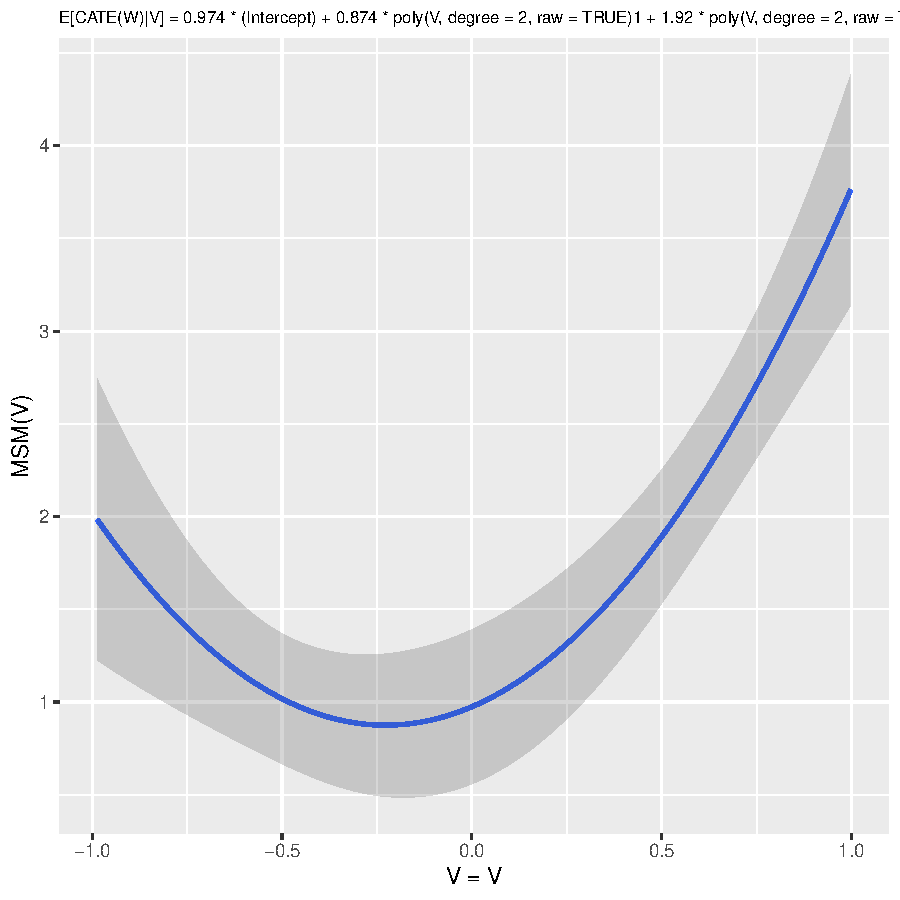
\includegraphics{causalglm-010}


\section{High dimensional semiparametric glms using the LASSO with causalglmnet}
In high dimensional settings (e.g. dim(W) >= 50-1000), conventional machine-learning algorithms may be computationally expensive or poorly behaved. In such scenarios, we can utilize lasso-penalized regression (Tibshirani, 1994) to estimate the nuisance parameters, allowing for adaptive variable selection and adjusting of confounders. The function causalglmnet is a specialized wrapper for spglm that uses the lasso implementation provided by the state-of-the-art R package glmnet (Friedman, 2010) for estimation of all nuisance parameters.\nocite{Friedman2010}\nocite{Tibshirani94regressionshrinkage} Its use is exactly the same as spglm except learners no longer need to be specified.

\begin{Schunk}
\begin{Sinput}
> n <- 200
> W <- replicate(100, runif(n, min = -1, max = 1))
> colnames(W) <- paste0("W", 1:100)
> beta <- runif(10, -1, 1) / 20
> A <- rbinom(n, size = 1, prob = plogis(W[, 10 * (1:10)] %*% beta))
> # CATE
> Y <- rnorm(n, mean = A + W[, 10 * (1:10)] %*% beta, sd = 0.5)
> data <- data.frame(W, A, Y)
> formula <- ~1
> output <-
+   causalglmnet(
+     formula,
+     data,
+     W = colnames(W), A = "A", Y = "Y",
+     estimand = "CATE",
+     verbose = FALSE
+   )
> summary(output)
> # OR
> Y <- rbinom(n, size = 1, prob = plogis(A + W[, 10 * (1:10)] %*% beta))
> data <- data.frame(W, A, Y)
> formula <- ~1
> output <-
+   causalglmnet(
+     formula,
+     data,
+     W = colnames(W), A = "A", Y = "Y",
+     estimand = "OR",
+     verbose = FALSE
+   )
> summary(output)
> # RR
> Y <- rpois(n, lambda = exp(A + W[, 10 * (1:10)] %*% beta))
> data <- data.frame(W, A, Y)
> formula <- ~1
> output <-
+   causalglmnet(
+     formula,
+     data,
+     W = colnames(W), A = "A", Y = "Y",
+     estimand = "RR",
+     verbose = FALSE
+   )
> summary(output)
> head(predict(output, data = data))
> 
\end{Sinput}
\end{Schunk}



\section{Robust nonparametric inference for the hazard ratio with npcoxph}
This is in development. \nocite{vanderLaanetal2007}


\bibliography{ref}

\end{document}
